% Sinh boi runners/make_paper1_figures.py; caption doi chieu bang
% runners/audit_figures.py. File rieng cho tung hinh de \input DUNG CHO
% trong than bai -- float cua LaTeX chi troi VE SAU, khai bao het o cuoi
% tai lieu thi ca 9 hinh don xuong cuoi va tran vao danh muc tai lieu.

\begin{figure*}[t]
  \centering
  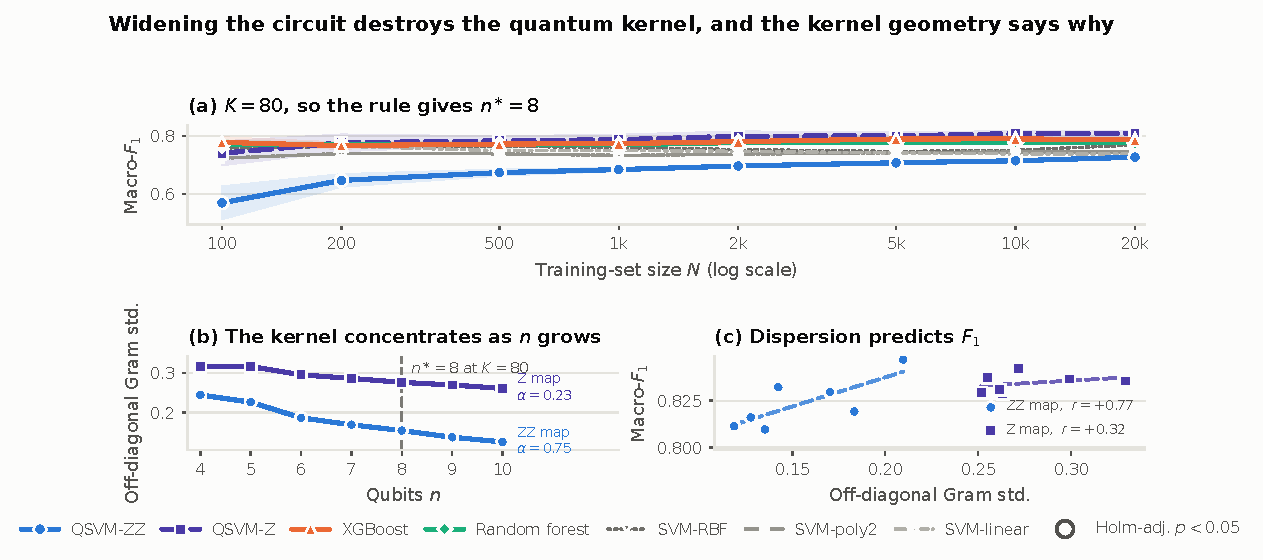
\includegraphics[width=\textwidth]{figs_revision/fig12_width_concentration.pdf}
  \caption{%
    \textbf{Widening the circuit destroys the quantum kernel, and the kernel
    geometry says why.} (a) The sample-complexity sweep re-run at $K=80$, where
    the rule returns $n^{\ast}=8$: all $48$ paired comparisons are
    classical-favourable. (b) Off-diagonal Gram dispersion against width, fitted
    as $n^{-\alpha}$; the \ZZ{} map concentrates about twice as fast as the
    \Zmap{} map. (c) That dispersion predicts macro-$F_1$ for \ZZ{}
    ($r=+0.77$) but not for \Zmap{} ($r=+0.32$).}
  \label{fig:width}
\end{figure*}
